% IEEE BDDM 2026 manuscript (integrated draft, 2026-11-14), five-page version.
% Red bracketed text marks items the author group must confirm before submission.
% Build: sh paper/latex/build.sh   (or: pdflatex main && bibtex main && pdflatex main && pdflatex main)
% The file compiles both inside this repository and from a flat folder that holds main.tex,
% IEEEctl.bib, references.bib and the two figure PDFs.
\documentclass[conference]{IEEEtran}
\IEEEoverridecommandlockouts

\usepackage[T1]{fontenc}
\usepackage{amsmath}
\usepackage{graphicx}
\usepackage{booktabs}
\usepackage{array}
\usepackage{xcolor}
\usepackage{cite}
\usepackage[hidelinks]{hyperref}
\usepackage{url}

\graphicspath{{../camera-ready/}{./}}
\newcommand{\confirm}[1]{\textcolor{red}{[#1]}}
\newcommand{\pp}{\,pp}
\newcommand{\pmean}{\bar{p}}

\begin{document}
\bstctlcite{IEEEctl:BSTcontrol}

\title{Imputation Disagreement for Selective Prediction with Missing Clinical Data: A Two-Hospital Reliability Evaluation}

\author{\IEEEauthorblockN{\confirm{Author names to be confirmed}}
\IEEEauthorblockA{\confirm{Affiliations and corresponding author to be confirmed}\\
\confirm{Email}}}

\maketitle

\begin{abstract}
Multiple imputation yields several predictions for each patient with incomplete measurements, and their disagreement is an appealing signal for selective prediction. We evaluated it in a matched design on the PhysioNet 2019 two-hospital cohort (24,095 patients, 95 with dataset-defined sepsis onset in intensive care unit hours 12--24). Confidence, missingness burden and imputation disagreement ranked the same logistic-regression predictions and the same split-conformal singleton pool at a 60\% acceptance target. First, marginal coverage hid a class-specific failure: set coverage was 90.75\% internally and 97.24\% externally, yet no positive patient's set contained the true label (0/8 and 0/38), because the pooled threshold admitted the positive label only above a predicted risk of 0.989. Second, at equal capacity disagreement showed no stable advantage over confidence: the selective-risk difference was $+0.109$ percentage points internally (95\% paired bootstrap interval $[0.000, +0.328]$) and $-0.036$ externally ($[-0.108, +0.036]$), and every ranking fell within the range of a uniform random ranking. Third, thresholds frozen in the source hospital did not transfer: external acceptance was 89.05\%, 86.09\% and 41.43\% for confidence, disagreement and missingness instead of 60\%. The prespecified conditional-increment model could not be fitted. Class-specific coverage, paired dispositions, a random-ranking reference and realized acceptance exposed failures that aggregate coverage concealed.
\end{abstract}

\begin{IEEEkeywords}
selective prediction, conformal prediction, multiple imputation, missing data, sepsis, reliability evaluation
\end{IEEEkeywords}

\section{Introduction}

Intensive care measurements are collected asynchronously and incompletely, so a model that predicts deterioration from the first 12 hours depends on how missing values are handled. Multiple imputation represents uncertainty about missing values instead of committing to one completed dataset~\cite{rubin1987multiple,vanbuuren2011mice}. A by-product is that predictions vary across plausible completions: two patients with the same mean predicted risk may differ in how sensitive that risk is to the completion. This imputation disagreement is an intuitive signal for deciding which predictions to act on automatically.

Selective prediction defers uncertain cases to human review~\cite{chow1970optimum,geifman2017selective,mozannar2020consistent}, and conformal prediction supplies prediction sets with distribution-free marginal coverage~\cite{angelopoulos2023conformal}, with recent extensions to clinical triage~\cite{kwon2026conformal} and to missing data~\cite{zaffran2023conformal,he2026safeimpute,wong2026mc2}. These studies do not settle whether imputation disagreement adds anything, as a ranking signal, to two signals that are available at no cost: the model's own confidence and the amount of missing data.

A fair answer requires a matched comparison: if rankings accept different numbers of patients or choose from different pools, differences in error cannot be attributed to the signal. With a rare outcome, aggregate coverage and error can also look reassuring while every positive patient is handled badly. We therefore ask three questions on a two-hospital sepsis cohort (Fig.~\ref{fig:pipeline}). \textbf{Q1:} How does overall prediction-set coverage relate to coverage and disposition among positive patients? \textbf{Q2:} With predictions, candidate pool and number accepted held fixed, how does replacing confidence with imputation disagreement change selective risk and individual dispositions? \textbf{Q3:} How much of the source-hospital acceptance capacity is retained when the same thresholds are applied at another hospital? Our contributions are as follows.
\begin{itemize}
\item \textbf{A matched evaluation protocol.} Confidence, missingness burden and imputation disagreement rank the same singleton pool under the same predictor, imputation draws, conformal threshold and acceptance count, so that differences in selective risk are attributable to the ranking alone; a uniform random ranking of the pool is the reference.
\item \textbf{Patient-level failure reporting.} Class-specific coverage and paired dispositions of positive patients show that 97\% aggregate coverage coexisted with exclusion of the true label for every external positive patient, and we trace this to the pooled conformal threshold.
\item \textbf{Evidence on threshold transfer.} Thresholds selected in one hospital for a 60\% target accepted between 41\% and 89\% of patients in the other hospital, depending on the signal.
\end{itemize}
The study evaluates reliability failure modes in a low-prevalence setting; its main result for imputation disagreement is negative.

\section{Related Work}

Split conformal prediction constructs prediction sets with finite-sample marginal coverage under exchangeability~\cite{angelopoulos2023conformal,vovk2005algorithmic}. Marginal coverage can be dominated by the majority class; label-conditional (Mondrian) calibration targets coverage within each class~\cite{vovk2005algorithmic,sadinle2019least}. Departures from exchangeability require weighting or explicit bounds~\cite{tibshirani2019covariate,barber2023beyond}. Selective classification trades coverage for risk by abstaining~\cite{chow1970optimum,geifman2017selective}, and learning-to-defer methods train the deferral rule jointly with the classifier~\cite{mozannar2020consistent}. Clinical triage studies combine conformal sets with cost-aware deferral~\cite{kwon2026conformal}, and Li et al.\ pair patient dispositions to study release-side risk under prevalence shift with target-site calibration subsets~\cite{li2026deployment}. Here the rankings share the source model and singleton pool, and source thresholds are applied externally without recalibration.

Multiple imputation propagates uncertainty about missing values into downstream estimates~\cite{rubin1987multiple,little2019statistical}, with chained equations as a standard implementation~\cite{vanbuuren2011mice}. Prior work studies conformal validity with imputed covariates~\cite{zaffran2023conformal}, controls the false discovery rate of released imputed values~\cite{he2026safeimpute}, calibrates by available modality~\cite{wong2026mc2}, or estimates uncertainty within a sequence model~\cite{vavaroutas2025squiredl}. Our unit of selection is a patient classification, and disagreement measures variation in that patient's predicted risk across imputations of a shared tabular predictor.

\section{Methods}

\begin{figure*}[t]
\centering
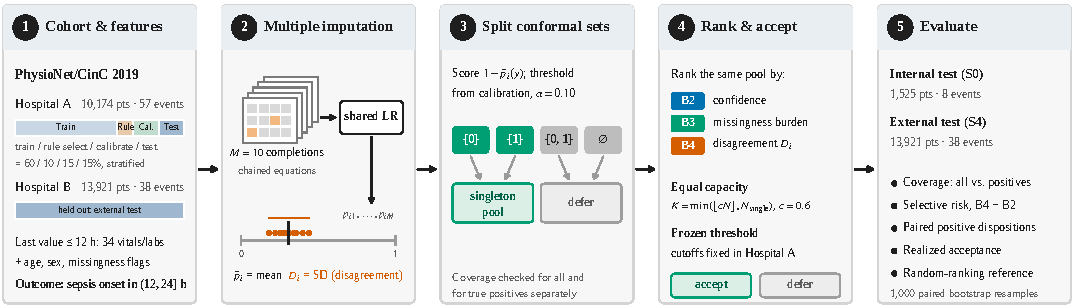
\includegraphics[width=\textwidth]{fig_pipeline.pdf}
\caption{Study pipeline. Hospital A provides the training, rule-selection, calibration and internal-test partitions and Hospital B the external test set. All rankings share the predictor, the $M=10$ imputation draws, the conformal threshold ($\alpha=0.10$) and the singleton pool; only the ranking signal differs.}
\label{fig:pipeline}
\end{figure*}

\subsection{Cohort, Labels and Partitions}
We use training sets A and B of the PhysioNet/Computing in Cardiology Challenge 2019~\cite{reyna2020early,goldberger2000physiobank}, each from a different hospital system; their sepsis labels follow the Sepsis-3 definition~\cite{singer2016sepsis3}. Eligible records contain intensive care unit (ICU) hours 1 through 24, and features use observations through hour 12. The challenge label turns positive six hours before the dataset-defined onset, so for records with an observed 0-to-1 transition we add six hours to the first positive label to recover the onset. We exclude records that are positive at the first observation, for which onset cannot be localized, and patients with onset by hour 12. The outcome is positive when the recovered onset falls after hour 12 and through hour 24.

Hospital A is split at the patient level into training (60\%), rule selection (10\%), calibration (15\%) and internal test (15\%), stratified by outcome. Training fits the imputer and classifier, rule selection chooses the hyperparameter and acceptance cutoffs, and calibration sets the conformal quantile. Hospital B is held out as the external test set. Seeds 2026--2030 repeat the split; seed 2026 is primary.

\subsection{Multiple Imputation and Shared Predictor}
Each of 34 physiological and laboratory variables is represented by its most recent observed value through hour 12; age, recorded sex and a missingness indicator for each input are added. A stochastic chained-equation imputer~\cite{vanbuuren2011mice} with Bayesian ridge conditional models is fitted on the training inputs (ten iterations) and produces $M=10$ completions of every partition. Imputed values are clipped to the training range and observed values are preserved.

A single L2-regularized logistic regression on standardized inputs is trained on the $M$ completed copies with weight $1/M$ per copy. Its regularization parameter is chosen from $\{0.1, 1, 10\}$ by average precision on the rule-selection partition; a 300-tree random forest is a robustness check. Let $p_{i,m}$ denote the predicted outcome probability of patient $i$ on completion $m$. We summarize the $M$ predictions by their mean and sample standard deviation,
\begin{equation}
\pmean_i=\frac{1}{M}\sum_{m=1}^{M}p_{i,m},\quad
D_i=\Bigl(\frac{1}{M-1}\sum_{m=1}^{M}(p_{i,m}-\pmean_i)^2\Bigr)^{1/2},
\label{eq:summary}
\end{equation}
and call $D_i$ the imputation disagreement. Completions are never treated as independent patients.

\subsection{Conformal Sets, Acceptance Rules and Comparators}
For a candidate label $y\in\{0,1\}$, let $\pmean_i(1)=\pmean_i$ and $\pmean_i(0)=1-\pmean_i$. The nonconformity score is $1-\pmean_i(y)$, and the threshold $q$ is the $\lceil (n+1)(1-\alpha)\rceil$-th smallest score of the true labels of the $n$ calibration patients at $\alpha=0.10$ (infinite if the index exceeds $n$). The prediction set is $\Gamma_i=\{y: 1-\pmean_i(y)\le q\}$. Coverage is computed over all test patients, including those with empty sets. Only singleton sets enter the automatic pool, with their single label as the prediction; empty and two-label sets are deferred.

At a target acceptance fraction $c\in\{0.40, 0.60, 0.80\}$, equal-capacity (batch) allocation ranks the pool and accepts the top $K=\min(\lfloor cN\rfloor, N_{\mathrm{single}})$ patients, where $N$ is the size of the test cohort and $N_{\mathrm{single}}$ that of its singleton pool. Every ranking therefore accepts the same number of patients from the same pool; ties are broken by a fixed hash of the patient identifier. In the frozen-threshold evaluation, the score and hash cutoffs that realize the target on the rule-selection partition are stored and applied unchanged to each test singleton, so realized acceptance can differ across signals and sites.

B1 accepts every singleton and shows the pool before ranking. Three signals rank the pool in ascending order: confidence (B2), $1-\max(\pmean_i, 1-\pmean_i)$; missingness burden (B3), the fraction of the 34 variables that are missing; and imputation disagreement (B4), $D_i$. B5 and B6 are prespecified error-risk models (L2 logistic regression, $C=1$) fitted on the rule-selection partition to predict the base classification error at $\pmean_i\ge 0.5$ from the B2 and B3 scores; B6 adds $D_i$, and B6 minus B5 is the conditional-increment contrast. They are fitted only if the partition contains at least 20 errors and 20 correct predictions.

\subsection{Metrics, Uncertainty and Sensitivity Analyses}
Acceptance is the number of accepted patients divided by all test patients. Selective risk is the number of accepted patients whose prediction is wrong divided by the number accepted. False-negative acceptances are true positives accepted with a negative prediction. The primary contrast is the selective risk of B4 minus that of B2 at $c=0.60$, in percentage points (pp).

Intervals are percentiles of 1,000 paired patient-level bootstrap resamples of the evaluation cohort with predictor and calibration fixed. Ranking and capacity are recomputed in each equal-capacity resample. Intervals for positive-class coverage are exact binomial. As a post hoc reference, we consider drawing $K$ patients uniformly without replacement from the singleton pool; the number of false-negative acceptances is then hypergeometric, and we report its expectation and central 95\% range. This range describes random allocation from the observed pool and is not a significance test.

S0 denotes the internal test set and S4 the external hospital, both under natural missingness. S1 and S2 additionally hide 10\% and 30\% of the observed physiological values at test time, and S3 hides the laboratory block; training and calibration are unchanged. Further checks use the random forest (S0, S2), $M=5$ and 20 (S0), $\alpha=0.05$ (S0, S2) and five test-time imputation batches, from which we compute how often a patient's decision differs between two batches. An independent implementation recomputed the reported coverage, paired dispositions and intervals.

\section{Results}

\subsection{Cohort and Base-Model Discrimination}
The source contained 40,336 records, of which 24,095 were eligible: 10,174 of 20,336 in Hospital A and 13,921 of 20,000 in Hospital B. A replay of all source records found 486 label transitions whose recovered onset fell in the target window (334 and 152). Of these, 102 were lost because the record did not start at ICU hour 1 and 289 because it ended before hour 24. The 95 retained events (57 and 38) are 19.5\% of the transitions and 0.39\% of eligible patients. The primary Hospital A split contained 6,104 training, 1,018 rule-selection, 1,527 calibration and 1,525 internal-test patients, with 34, 6, 9 and 8 events.

The selected logistic regression ($C=0.1$) reached an AUROC of 0.793 internally (95\% interval $[0.579, 0.947]$) and 0.502 externally ($[0.407, 0.596]$). Average precision was 0.029 and 0.0029 against prevalences of 0.52\% and 0.27\%. The random-forest diagnostic reached an external AUROC of 0.581 ($[0.480, 0.674]$). Discrimination was thus moderate but imprecise internally and close to chance externally.

\subsection{Marginal Coverage Hid the Loss of Every Positive}
Overall set coverage was 1,384/1,525 (90.75\%) internally and 13,537/13,921 (97.24\%) externally, at or above the nominal 90\%. Positive-class coverage was 0/8 and 0/38 (Fig.~\ref{fig:reliability}a). With 9 positives among 1,527 calibration patients, the pooled threshold was $q=0.011$, so the negative label entered a set whenever $\pmean_i\le 0.011$ and the positive label only when $\pmean_i\ge 0.989$. Predicted risks were nowhere near that level: the largest $\pmean_i$ among test positives was 0.023 internally and 0.0075 externally. Four internal positives exceeded 0.011 and received empty sets; the other four, and all 38 external positives, became negative singletons and entered the automatic pool.

No positive singleton occurred, so all accepted predictions were negative: selective risk equals the false-negative rate among accepted patients, and automatic acceptance acted as rule-out triage. Accepting every singleton (B1) would have released 1,388 internal patients including 4 of the 8 positives, and 13,575 external patients (97.51\%) including all 38 positives (Table~\ref{tab:main}).

\begin{figure*}[t]
\centering
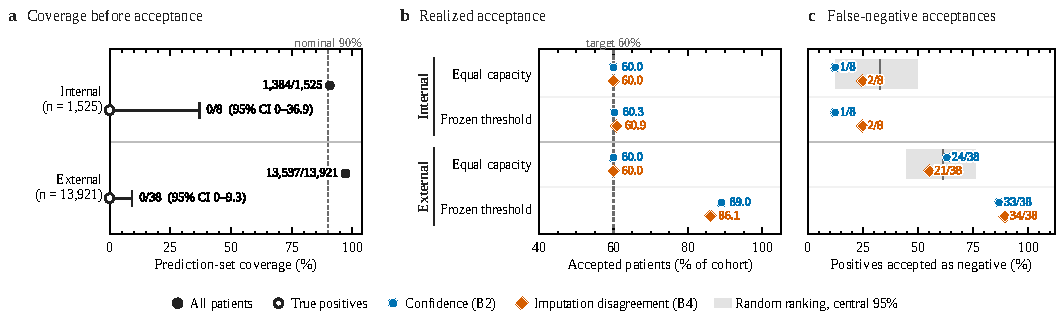
\includegraphics[width=\textwidth]{fig1_reliability.pdf}
\caption{Prediction-set coverage and patient disposition (logistic regression, seed 2026, $M=10$, $\alpha=0.10$, 60\% target). (a) Set coverage with exact 95\% binomial intervals; the dashed line marks the nominal 90\%. (b) Accepted share of the test cohort at equal capacity and with thresholds frozen in the source hospital. (c) Positives accepted as negative; grey bands and ticks show the central 95\% range and expectation of a uniform random ranking of the same pool.}
\label{fig:reliability}
\end{figure*}

\begin{table}[t]
\caption{Acceptance and False-Negative Acceptances at the 60\% Target}
\label{tab:main}
\centering
\footnotesize
\setlength{\tabcolsep}{4pt}
\begin{tabular}{@{}lcccc@{}}
\toprule
 & \multicolumn{2}{c}{Internal (S0)} & \multicolumn{2}{c}{External (S4)} \\
\cmidrule(lr){2-3}\cmidrule(l){4-5}
Strategy & Acc.\ (\%) & Missed & Acc.\ (\%) & Missed \\
\midrule
\multicolumn{5}{@{}l}{\emph{Without ranking}} \\
B1 All singletons & 91.02 & 4/8 & 97.51 & 38/38 \\
\multicolumn{5}{@{}l}{\emph{Equal capacity ($K=915$ and $8{,}352$)}} \\
B2 Confidence & 60.00 & 1/8 & 60.00 & 24/38 \\
B3 Missingness & 60.00 & 2/8 & 60.00 & 24/38 \\
B4 Disagreement & 60.00 & 2/8 & 60.00 & 21/38 \\
Random ranking & 60.00 & 2.64 (1--4) & 60.00 & 23.38 (17--29) \\
\multicolumn{5}{@{}l}{\emph{Thresholds frozen in Hospital A}} \\
B2 Confidence & 60.26 & 1/8 & 89.05 & 33/38 \\
B3 Missingness & 60.00 & 2/8 & 41.43 & 19/38 \\
B4 Disagreement & 60.85 & 2/8 & 86.09 & 34/38 \\
\bottomrule
\end{tabular}

\smallskip
\parbox{\columnwidth}{\scriptsize Acc.: accepted share of the cohort. Missed: positives accepted as negative. Random: mean (central 95\% range).}
\end{table}

\subsection{Equal-Capacity Ranking and Paired Dispositions}
At the 60\% target, each ranking accepted 915 internal and 8,352 external patients (Table~\ref{tab:main}). Internally, confidence accepted one positive as negative and disagreement two, a selective-risk difference of $+0.109$\pp{} (95\% paired bootstrap interval $[0.000, +0.328]$); missingness also accepted two. Externally, confidence and missingness each accepted 24 of the 38 positives and disagreement 21, a difference of $-0.036$\pp{} ($[-0.108, +0.036]$). A uniform random ranking of the same pools would accept 2.64 and 23.38 positives on average, with central 95\% ranges of 1--4 and 17--29, and all three rankings fell inside these ranges at both hospitals (Fig.~\ref{fig:reliability}c).

The external net reduction of three false-negative acceptances was not a uniform improvement. Relative to confidence, disagreement deferred six positives and newly accepted three others, while 18 positives were accepted as negative by both rankings and 11 were deferred by both. Internally, one positive was missed by both rankings, one by disagreement only, and six were deferred by both. The rule-selection partition contained six classification errors and 1,012 correct classifications, below the minimum of 20 errors, so B5 and B6 could not be fitted. The prespecified conditional increment of disagreement beyond confidence and missingness is therefore not estimable.

\subsection{Threshold Transfer}
On the internal test set, the frozen cutoffs accepted 60.26\% (confidence), 60.00\% (missingness) and 60.85\% (disagreement) of patients. On the external hospital, they accepted 89.05\%, 41.43\% and 86.09\% (Fig.~\ref{fig:reliability}b, Table~\ref{tab:main}). The confidence and disagreement rules thereby released 33 and 34 of the 38 external positives, more than at equal capacity, whereas the missingness rule released 19 while accepting far fewer patients than intended. Across the five splits, external acceptance was 79.48--89.54\% for confidence and 72.33--86.29\% for disagreement, above the target in every split.

\subsection{Sensitivity and Stability}
Across the five seeds, the equal-capacity difference between disagreement and confidence ranged from $-0.109$ to $+0.109$\pp{} internally and from $-0.048$ to $+0.012$\pp{} externally, and it was zero for every seed under 30\% additional masking (S2). In the prespecified random-forest, $M$ and $\alpha$ checks it ranged from $0.000$ to $+0.219$\pp{}, and every 95\% interval reached zero. Disagreement was also the least reproducible ranking: between pairs of imputation batches, the decision changed for 17.18\% of patients on average, compared with 4.79\% under confidence and 0.79\% under missingness.

\section{Discussion}

High aggregate coverage coexisted with exclusion of the true label from every positive patient's prediction set. Split conformal coverage is a marginal guarantee under exchangeability; when positives are 0.3--0.6\% of the cohort, it can be met by covering negatives alone, and here it was. The candidate pool then consisted entirely of negative predictions, so every ranking signal was choosing which rule-outs to release, not which predictions to trust.

Label-conditional (Mondrian) calibration is the natural remedy, because it sets a separate threshold for each label~\cite{vovk2005algorithmic,sadinle2019least}. Here it faces a sample-size constraint: the calibration partition held nine positives, so at $\alpha=0.10$ the positive-class threshold would equal the lowest predicted risk among them. With limited discrimination, such a threshold would add the positive label to many negative patients' sets and shrink the singleton pool. We did not evaluate it; a credible assessment needs more calibration events.

At equal capacity, disagreement and confidence changed which patients were accepted but not, in any stable way, how many positives were missed. The differences amount to one patient internally and three externally, their direction differed between hospitals and across splits, and none of the three signals fell outside the range expected from ranking the pool at random. With an external AUROC of 0.502, the external comparison contrasts orderings of a predictor that barely separates outcomes; we read it as evidence about failure under transfer, not about the quality of the signals. Disagreement also changed the decision of about one patient in six between imputation batches.

Frozen cutoffs added a second transfer failure. The thresholds that met the 60\% target internally accepted between 41\% and 89\% of external patients, so neither the review workload nor the number of released positives was controlled. Four reporting practices made these failures visible, and we recommend them for selective prediction with rare outcomes: (i) coverage by outcome class, with counts; (ii) the composition of the candidate pool, including whether any positive prediction can be accepted at all; (iii) paired dispositions of positive patients and a random-ranking reference at the same capacity; and (iv) realized acceptance when a rule is moved to another site.

The study has clear limits. Only 95 events were available, eight in the internal test set, so one patient moves any internal positive-class rate by 12.5 percentage points. The prespecified conditional-increment analysis could not be performed. Eligibility required 24 hours of recorded follow-up, which removed about four fifths of the target-window transitions, and the endpoint relies on the dataset's onset definition and a fixed label offset. One retrospective dataset and one held-out hospital were reused across splits. The paired dispositions and the random reference were added after inspection of the primary results. We evaluated neither class-conditional calibration nor a stronger base model, and clinical conclusions would require prospective data.

\section{Conclusion}

In a matched two-hospital evaluation, ranking conformal singletons by imputation disagreement gave no stable reduction in selective risk relative to confidence, and no signal fell outside the range of a random ranking of the same pool. Marginal coverage of 91--97\% concealed zero coverage of positive patients, and thresholds frozen in the source hospital accepted 41--89\% of external patients instead of 60\%. For rare outcomes, class-specific coverage, pool composition, paired dispositions and realized acceptance should be reported alongside aggregate coverage and risk.

\section*{Data Availability and Ethics}
The PhysioNet/Computing in Cardiology Challenge 2019 data are publicly available from PhysioNet (\url{https://physionet.org/content/challenge-2019/1.0.0/}). We do not redistribute patient-level records or derived patient-level files. Aggregate results and analysis code are available from the authors \confirm{public repository or on request}. This secondary analysis of a public, de-identified dataset required no additional ethical approval \confirm{confirm against institutional policy}.

\section*{Acknowledgment}
\confirm{Authors to confirm tools and scope:} Generative AI tools (OpenAI Codex and Anthropic Claude) assisted with code review, cross-checking numeric statements against the experiment records, figure preparation and language editing. The authors reviewed all content and take full responsibility for it. \confirm{Add funding information, if any.}

\bibliographystyle{IEEEtran}
\IfFileExists{references.bib}{\bibliography{IEEEctl,references}}{\bibliography{IEEEctl,../references}}

\end{document}
